\let\negmedspace\undefined
\let\negthickspace\undefined
\documentclass[journal,12pt,onecolumn]{IEEEtran}
\usepackage{cite}
\usepackage{amsmath,amssymb,amsfonts,amsthm}
\usepackage{algorithmic}
\usepackage{graphicx}
\graphicspath{{./figs/}}
\usepackage{textcomp}
\usepackage{xcolor}
\usepackage{txfonts}
\usepackage{listings}
\usepackage{enumitem}
\usepackage{mathtools}
\usepackage{gensymb}
\usepackage{comment}
\usepackage{mhchem}
\usepackage{caption}
\usepackage[breaklinks=true]{hyperref}
\usepackage{tkz-euclide} 
\usepackage{listings}
\usepackage{gvv}                                        
%\def\inputGnumericTable{}                                   
\usepackage[utf8]{inputenc}     
\usepackage{xparse}
\usepackage{color}                                            
\usepackage{array}                                            
\usepackage{longtable}                                       
\usepackage{calc}                                             
\usepackage{multirow}
\usepackage{multicol}
\usepackage{hhline}                                           
\usepackage{ifthen}                                           
\usepackage{lscape}
\usepackage{tabularx}
\usepackage{array}
\usepackage{float}
\newtheorem{theorem}{Theorem}[section]
\newtheorem{problem}{Problem}
\newtheorem{proposition}{Proposition}[section]
\newtheorem{lemma}{Lemma}[section]
\newtheorem{corollary}[theorem]{Corollary}
\newtheorem{example}{Example}[section]
\newtheorem{definition}[problem]{Definition}
\newcommand{\BEQA}{\begin{eqnarray}}
\newcommand{\EEQA}{\end{eqnarray}}
\newcommand{\define}{\stackrel{\triangle}{=}}
\theoremstyle{remark}
\newtheorem{rem}{Remark}

\usepackage{enumitem}
\setlist[enumerate,1]{label=\arabic*.}
\setlist[enumerate,2]{label=(\Alph*)}


\begin{document}

\title{
 GATE 2014 \\
XL: Life Sciences}
\author{EE25BTECH11049 - Sai Krishna Bakki}
\date{}
\maketitle

\begin{enumerate}
    \item The movie was funny and I \underline{\hspace{2cm}}.

    \hfill{\brak{\text{GATE XL 2022}}}
    \begin{enumerate}
        \begin{multicols}{2}
            \item could help laughing
            \item couldn't help laughed
            \item couldn't help laughing
            \item could helped laughed
        \end{multicols}
    \end{enumerate}

    \item $x \colon y \colon z = \frac{1}{2} \colon \frac{1}{3} \colon \frac{1}{4}$. What is the value of $\frac{x+z-y}{y}$?

    \hfill{\brak{\text{GATE XL 2022}}}
    \begin{enumerate}
        \begin{multicols}{4}
            \item $0.75$
            \item $1.25$
            \item $2.25$
            \item $3.25$
        \end{multicols}
    \end{enumerate}

    \item Both the numerator and the denominator of $\frac{3}{4}$ are increased by a positive integer, $x$, and those of $\frac{15}{17}$ are decreased by the same integer. This operation results in the same value for both the fractions. What is the value of $x$?

    \hfill{\brak{\text{GATE XL 2022}}}
    \begin{enumerate}
        \begin{multicols}{4}
            \item $1$
            \item $2$
            \item $3$
            \item $4$
        \end{multicols}
    \end{enumerate}

    \item A survey of $450$ students about their subjects of interest resulted in the following outcome.
    \begin{itemize}
        \item $150$ students are interested in Mathematics.
        \item $200$ students are interested in Physics.
        \item $175$ students are interested in Chemistry.
        \item $50$ students are interested in Mathematics and Physics.
        \item $60$ students are interested in Physics and Chemistry.
        \item $40$ students are interested in Mathematics and Chemistry.
        \item $30$ students are interested in Mathematics, Physics and Chemistry.
        \item Remaining students are interested in Humanities.
    \end{itemize}
    Based on the above information, the number of students interested in Humanities is

    \hfill{\brak{\text{GATE XL 2022}}}
    \begin{enumerate}
        \begin{multicols}{4}
            \item $10$
            \item $30$
            \item $40$
            \item $45$
        \end{multicols}
    \end{enumerate}

    \item For the picture shown above, which one of the following is the correct picture representing reflection with respect to the mirror shown as the dotted line?
    \begin{figure}[H]
        \centering
        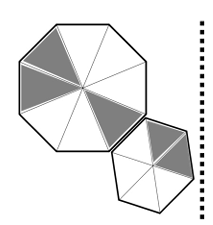
\includegraphics[width=0.2\columnwidth]{fig1.png}
        \caption*{}
        \label{fig:q5}
    \end{figure}

    \hfill{\brak{\text{GATE XL 2022}}}
    \begin{enumerate}
    \begin{multicols}{2}
        \begin{figure}[H]
            \centering
         \item   \begin{minipage}{0.45\textwidth}
                \centering
                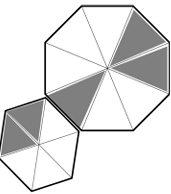
\includegraphics[width=0.2\columnwidth]{fig2.png}
                \caption*{}
                \label{fig:a5a}
            \end{minipage}
         \item    \begin{minipage}{0.45\textwidth}
                \centering
                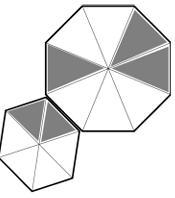
\includegraphics[width=0.2\columnwidth]{fig3.png}
                \caption*{}
                \label{fig:a5b}
            \end{minipage}
    \item         \begin{minipage}{0.45\textwidth}
                \centering
                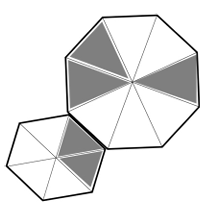
\includegraphics[width=0.2\columnwidth]{fig4.png}
                \caption*{}
                \label{fig:a5c}
            \end{minipage}
      \item       \begin{minipage}{0.45\textwidth}
                \centering
                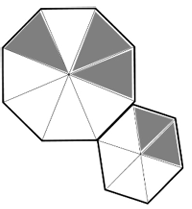
\includegraphics[width=0.2\columnwidth]{fig5.png}
                \caption*{}
                \label{fig:a5d}
            \end{minipage}
        \end{figure}
           \end{multicols}
    \end{enumerate}

    \item In the last few years, several new shopping malls were opened in the city. The total number of visitors in the malls is impressive. However, the total revenue generated through sales in the shops in these malls is generally low. Which one of the following is the CORRECT logical inference based on the information in the above passage?

    \hfill{\brak{\text{GATE XL 2022}}}
    \begin{enumerate}
        \item Fewer people are visiting the malls but spending more
        \item More people are visiting the malls but not spending enough
        \item More people are visiting the malls and spending more
        \item Fewer people are visiting the malls and not spending enough
    \end{enumerate}

    \item In a partnership business the monthly investment by three friends for the first six months is in the ratio $3 \colon 4 \colon 5$. After six months, they had to increase their monthly investments by $10\%$, $15\%$ and $20\%$, respectively, of their initial monthly investment. The new investment ratio was kept constant for the next six months. What is the ratio of their shares in the total profit \brak{\text{in the same order}} at the end of the year such that the share is proportional to their individual total investment over the year?

    \hfill{\brak{\text{GATE XL 2022}}}
    \begin{enumerate}
        \begin{multicols}{2}
            \item $22 \colon 23 \colon 24$
            \item $22 \colon 33 \colon 50$
            \item $33 \colon 46 \colon 60$
            \item $63 \colon 86 \colon 110$
        \end{multicols}
    \end{enumerate}

    \item Consider the following equations of straight lines:
    \begin{align*}
        \text{Line L1} &\colon 2x - 3y = 5 \\
        \text{Line L2} &\colon 3x + 2y = 8 \\
        \text{Line L3} &\colon 4x - 6y = 5 \\
        \text{Line L4} &\colon 6x - 9y = 6
    \end{align*}
    Which one among the following is the correct statement?

    \hfill{\brak{\text{GATE XL 2022}}}
    \begin{enumerate}
        \item L1 is parallel to L2 and L1 is perpendicular to L3
        \item L2 is parallel to L4 and L2 is perpendicular to L1
        \item L3 is perpendicular to L4 and L3 is parallel to L2
        \item L4 is perpendicular to L2 and L4 is parallel to L3
    \end{enumerate}

    \item Given below are two statements and four conclusions drawn based on the statements.
    \begin{itemize}
        \item[] Statement 1: Some soaps are clean.
        \item[] Statement 2: All clean objects are wet.
    \end{itemize}
    \begin{itemize}
        \item[] Conclusion I: Some clean objects are soaps.
        \item[] Conclusion II: No clean object is a soap.
        \item[] Conclusion III: Some wet objects are soaps.
        \item[] Conclusion IV: All wet objects are soaps.
    \end{itemize}
    Which one of the following options can be logically inferred?

    \hfill{\brak{\text{GATE XL 2022}}}
    \begin{enumerate}
        \item Only conclusion I is correct
        \item Either conclusion I or conclusion II is correct
        \item Either conclusion III or conclusion IV is correct
        \item Only conclusion I and conclusion III are correct
    \end{enumerate}

    \item An ant walks in a straight line on a plane leaving behind a trace of its movement. The initial position of the ant is at point P facing east. The ant first turns $72\degree$ anticlockwise at P, and then does the following two steps in sequence exactly FIVE times before halting.
    \begin{enumerate}
        \item moves forward for 10 cm.
        \item turns $144\degree$ clockwise.
    \end{enumerate}
    The pattern made by the trace left behind by the ant is
    \begin{figure}[H]
        \centering
        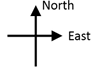
\includegraphics[width=0.2\linewidth]{fig6.png}
        \caption{}
        \label{fig:placeholder}
    \end{figure}

    \hfill{\brak{\text{GATE XL 2022}}}
    \begin{enumerate}
    \begin{multicols}{2}
         \begin{figure}[H]
    \item    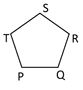
\includegraphics[width=0.15\columnwidth]{fig7.png} \caption*{} \label{fig:a10a} \end{figure}
         \begin{figure}[H] \item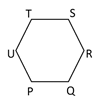
\includegraphics[width=0.15\columnwidth]{fig8.png} \caption*{} \label{fig:a10b} \end{figure}
         \begin{figure}[H] \item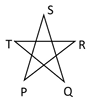
\includegraphics[width=0.15\columnwidth]{fig9.png} \caption*{} \label{fig:a10c} \end{figure}
         \begin{figure}[H] \item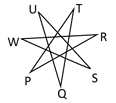
\includegraphics[width=0.15\columnwidth]{fig10.png} \caption*{} \label{fig:a10d} \end{figure}
         \end{multicols}
    \end{enumerate}
    
    \item Consider a second order reaction, $2A \rightarrow \text{Product}$. The concentration of A is represented as [A]. Which of the following is the CORRECT plot for determining the rate constant for the above reaction?

    \hfill{\brak{\text{GATE XL 2022}}}
    \begin{enumerate}
        \begin{figure}[h!]
            \centering
            \begin{minipage}{0.45\textwidth}
                \centering
         \item  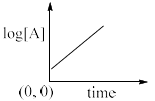
\includegraphics[width=0.8\linewidth]{fig11.png}
                \caption*{}
                \label{fig:a11a}
            \end{minipage}
            \begin{minipage}{0.45\textwidth}
                \centering
             \item   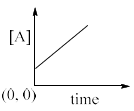
\includegraphics[width=0.8\linewidth]{fig12.png}
                \caption*{}
                \label{fig:a11b}
            \end{minipage}
            \begin{minipage}{0.45\textwidth}
                \centering
           \item     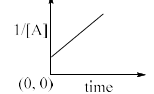
\includegraphics[width=0.8\linewidth]{fig13.png}
                \caption*{}
                \label{fig:a11c}
            \end{minipage}
            \begin{minipage}{0.45\textwidth}
                \centering
           \item     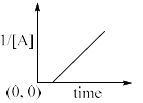
\includegraphics[width=0.8\linewidth]{fig14.png}
                \caption*{}
                \label{fig:a11d}
            \end{minipage}
        \end{figure}
    \end{enumerate}

    \item Which among the following has the least second ionization energy?

    \hfill{\brak{\text{GATE XL 2022}}}
    \begin{enumerate}
        \begin{multicols}{4}
            \item Al
            \item Si
            \item P
            \item S
        \end{multicols}
    \end{enumerate}

    \item Which among the following metal ions has the highest enthalpy of hydration? \brak{\text{Assume the given metal ions have the same counter ion.}} Given: Atomic numbers of Ti, V, Cr and Mn are 22, 23, 24 and 25, respectively.

    \hfill{\brak{\text{GATE XL 2022}}}
    \begin{enumerate}
        \begin{multicols}{4}
            \item Ti$^{2+}$
            \item V$^{2+}$
            \item Cr$^{2+}$
            \item Mn$^{2+}$
        \end{multicols}
    \end{enumerate}

    \item Among the following, the one having smallest bond angle is

    \hfill{\brak{\text{GATE XL 2022}}}
    \begin{enumerate}
        \begin{multicols}{4}
            \item PH$_3$
            \item PF$_3$
            \item NF$_3$
            \item NH$_3$
        \end{multicols}
    \end{enumerate}

    \item Which of the following is the CORRECT statement about hexoses?

    \hfill{\brak{\text{GATE XL 2022}}}
    \begin{enumerate}
        \item D-mannose is C-4 epimer of D-glucose
        \item D-galactose is C-2 epimer of D-glucose
        \item D-glucose and L-glucose are diastereomers
        \item D-glucose and D-galactose are diastereomers
    \end{enumerate}

    \item The bases present in DNA are

    \hfill{\brak{\text{GATE XL 2022}}}
    \begin{enumerate}
        \item adenine, cytosine, guanine and thymine
        \item adenine, guanine, thymine and uracil
        \item adenine, cytosine, thymine and uracil
        \item cytosine, guanine, thymine and uracil
    \end{enumerate}

    \item The CORRECT order of basicity for the following compounds is
    \begin{figure}[h!]
        \centering
        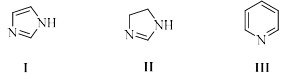
\includegraphics[width=0.5\columnwidth]{fig15.png}
        \caption*{}
        \label{fig:q17}
    \end{figure}

    \hfill{\brak{\text{GATE XL 2022}}}
    \begin{enumerate}
        \begin{multicols}{4}
            \item I \> II \> III
            \item II \> III \> I
            \item II \> I \> III
            \item III \> I \> II
        \end{multicols}
    \end{enumerate}

    \item Molar conductance of monobromoacetic acid at infinite dilution is calculated to be $x \times 10^{-4}$ S m$^2$ mol$^{-1}$ at $25\degree$C. The value of $x$ is \brak{\text{round off to the nearest integer}}.
    Given:
    \begin{table}[h!]
    \centering
    \caption*{}
    \label{tab:q18}
    \begin{tabular}{|l|c|}
    \hline
    \textbf{Electrolyte} & \textbf{Limiting molar conductance} \\
     & \textbf{at $25\degree$C in $10^{-4}$ S m$^2$ mol$^{-1}$} \\
    \hline
    HBr & $427.95$ \\
    KBr & $151.64$ \\
    CH$_2$BrCOOK & $112.72$ \\
    \hline
    \end{tabular}
    \end{table}

    \hfill{\brak{\text{GATE XL 2022}}}
    \begin{enumerate}
        \begin{multicols}{4}
            \item $164$
            \item $195$
            \item $389$
            \item $467$
        \end{multicols}
    \end{enumerate}

    \item A sample of benzene, contaminated with a non-volatile and non-ionic solute, boils at $0.31\degree$C higher than that of pure benzene. The molality of the solute in the contaminated solution is \underline{\hspace{2cm}} \brak{\text{round off to two decimal places}}.
    Given: Gas constant = $8.314$ J K$^{-1}$ mol$^{-1}$
    Molecular weight of benzene is $78.11$ g mol$^{-1}$
    Normal boiling point of benzene is $80.1\degree$C
    Enthalpy of vaporization of benzene is $30.76$ kJ mol$^{-1}$

    \hfill{\brak{\text{GATE XL 2022}}}

    \item Among the following statements about cobalt complexes, which is/are CORRECT?
    Given: Atomic number of Co is $27$

    \hfill{\brak{\text{GATE XL 2022}}}
    \begin{enumerate}  
        \item [Co(NH$_3$)$_4$]$^{2+}$ exhibits square planar geometry
        \item [Co(en)$_3$]$^{3+}$ does not show optical isomerism \brak{\text{en = ethylenediamine}}
        \item [Co(H$_2$O)$_6$]$^{3+}$ is paramagnetic in nature
        \item [Co(NH$_3$)$_5$Cl)]$^{2+}$ shows ligand-to-metal charge transfer
    \end{enumerate}

    \item Consider the following reaction:
    \begin{figure}[H]
        \centering
        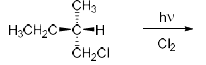
\includegraphics[width=0.3\columnwidth]{fig16.png}
        \caption*{}
        \label{fig:q21}
    \end{figure}
    The CORRECT statement\brak{\text{s}} related to mono-chlorination at carbon-2 position is/are

    \hfill{\brak{\text{GATE XL 2022}}}
    \begin{enumerate}
        \item The reaction proceeds through alkyl radical intermediate
        \item Complete inversion of configuration at carbon-2 takes place
        \item Complete retention of configuration at carbon-2 takes place
        \item A mixture of enantiomers is formed
    \end{enumerate}

    \item Consider the following enzyme catalyzed reaction:
    \[ E + S \rightleftharpoons ES \rightarrow P + E \]
    where E is enzyme, S is substrate, ES is enzyme-substrate complex and P is product.
    The CORRECT statement\brak{\text{s}} for the above reaction is/are

    \hfill{\brak{\text{GATE XL 2022}}}
    \begin{enumerate}
        \item Maximum possible rate of product formation is dependent on $k_2$ and initial concentration of enzyme.
        \item For a low substrate concentration, the rate of product formation is first order with respect to enzyme and also first order with respect to the substrate.
        \item The rate of product formation is independent of the concentration of enzyme substrate complex.
        \item For a very high substrate concentration, initial rate of product formation is zero order with respect to the substrate.
    \end{enumerate}

    \item Consider the following reaction:
    \begin{figure}[h!]
        \centering
        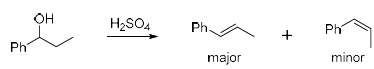
\includegraphics[width=0.6\columnwidth]{fig17.png}
        \caption*{}
        \label{fig:q23}
    \end{figure}
    The CORRECT pathway\brak{\text{s}} involved in the reaction is/are

    \hfill{\brak{\text{GATE XL 2022}}}
    \begin{enumerate}
        \item E2 followed by isomerization
        \item E1 followed by isomerization
        \item SN1 followed by isomerization
        \item Isomerization through carbocation
    \end{enumerate}

    \item An aqueous solution of aspirin \brak{\text{HA}} is prepared at pH $7.4$. The ratio of concentration of A$^-$ and HA at equilibrium is \underline{\hspace{2cm}} \brak{\text{round off to the nearest integer}}.
    Given: K$_a$ of aspirin is $3.98 \times 10^{-4}$

    \hfill{\brak{\text{GATE XL 2022}}}

    \item The total number of 3-centre-2-electron bonds in B$_4$H$_{10}$ is \underline{\hspace{2cm}} \brak{\text{in integer}}.

    \hfill{\brak{\text{GATE XL 2022}}}

    \item The equilibrium constant for isomerization of 1-butene to trans-2-butene at $27\degree$C is \underline{\hspace{2cm}} \brak{\text{round off to one decimal place}}.
    Given: Gas constant = $8.314$ J K$^{-1}$ mol$^{-1}$
    $\Delta_f G^o$ of 1-butene = $+71.39$ kJ mol$^{-1}$
    $\Delta_f G^o$ of trans-2-butene = $+63.06$ kJ mol$^{-1}$

    \hfill{\brak{\text{GATE XL 2022}}}

    \item A $16$ mW monochromatic light emits $4 \times 10^{16}$ photons in $1$ second. When this light incidents on a metal strip, photoelectrons are emitted. The wavelength of the emitted photoelectrons \brak{\text{in \AA}} is \underline{\hspace{2cm}} \brak{\text{round off to one decimal place}}.
    Given: Work function of the metal = $2.0$ eV
    Charge of an electron = $1.6 \times 10^{-19}$ C
    Mass of an electron = $9.1 \times 10^{-31}$ kg
    Planck's constant = $6.626 \times 10^{-34}$ J s

    \hfill{\brak{\text{GATE XL 2022}}}

     \item Which of the immune cells listed below are agranular?
    \begin{itemize}
        \item[P.] Eosinophils
        \item[Q.] Mast cells
        \item[R.] Monocytes
        \item[S.] T-cells
    \end{itemize}

    \hfill{\brak{\text{GATE XL 2022}}}
    \begin{enumerate}
        \begin{multicols}{2}
            \item P and Q only
            \item Q and R only
            \item R and S only
            \item S and P only
        \end{multicols}
    \end{enumerate}

    \item Which one of the following enzymes is located in the outer mitochondrial membrane?

    \hfill{\brak{\text{GATE XL 2022}}}
    \begin{enumerate}
        \begin{multicols}{2}
            \item Citrate synthase
            \item Fumarase
            \item Monoamine oxidase
            \item Succinate dehydrogenase
        \end{multicols}
    \end{enumerate}

    \item Which one of the following statements about the DNA polymerase III of E. coli is NOT correct?

    \hfill{\brak{\text{GATE XL 2022}}}
    \begin{enumerate}
        \item It catalyzes nick translation.
        \item Its absence is lethal to E. coli.
        \item It synthesizes a complementary DNA strand using a single-stranded template.
        \item It possesses $3' \rightarrow 5'$ exonuclease activity.
    \end{enumerate}

    \item Which one of the following compounds is NOT a translation inhibitor?

    \hfill{\brak{\text{GATE XL 2022}}}
    \begin{enumerate}
        \begin{multicols}{2}
            \item Chloramphenicol
            \item Cycloheximide
            \item Puromycin
            \item Rifampicin
        \end{multicols}
    \end{enumerate}

    \item A dye was allowed to undergo migration on a chromatographic paper using a solvent. The dye, and the solvent-front migrated $5$ and $20$ cm, respectively, from the point of origin. The retention factor \brak{\text{rounded off to two places of decimals}} for the dye is \underline{\hspace{2cm}}.

    \hfill{\brak{\text{GATE XL 2022}}}

    \item The $pK_a$ values of the carboxylic and amino groups of an amino acid with a non-ionizable side chain are $2.17$ and $9.13$, respectively. The isoelectric point \brak{\text{rounded off to two places of decimals}} of this amino acid is \underline{\hspace{2cm}}.

    \hfill{\brak{\text{GATE XL 2022}}}

    \item The number of ATP molecules required for the complete assimilation of one molecule of CO$_2$ in Calvin cycle is \underline{\hspace{2cm}}.

    \hfill{\brak{\text{GATE XL 2022}}}

    \item The absorbance of a $5 \times 10^{-4}$ M solution of tyrosine at $280$ nm wavelength is $0.75$. The path length of the cuvette is $1$ cm. The molar absorption coefficient at the given wavelength in M$^{-1}$cm$^{-1}$, correct to the nearest integer, is \underline{\hspace{2cm}}.

    \hfill{\brak{\text{GATE XL 2022}}}

    \item Filamentous photosynthetic algae were placed on a microscopic slide and illuminated with light of different colors as illustrated.
    \begin{figure}[h!]
        \centering
        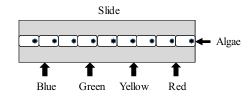
\includegraphics[width=0.6\columnwidth]{fig18.png}
        \caption*{}
        \label{fig:q36}
    \end{figure}
    The bacteria that are known to migrate towards the region of high $O_2$ were also added uniformly on the slide. Which one of the following options illustrates the distribution of bacteria along the length of the microscopic slide after illumination?

    \hfill{\brak{\text{GATE XL 2022}}}
    \begin{enumerate}
        \begin{figure}[h!]
            \centering
            \begin{minipage}{0.45\textwidth}
                \centering
       \item    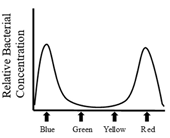
\includegraphics[width=\linewidth]{fig19.png}
                \caption*{}
                \label{fig:a36a}
            \end{minipage}%
            \begin{minipage}{0.45\textwidth}
                \centering
 \item        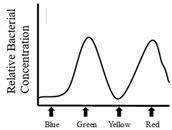
\includegraphics[width=\linewidth]{fig20.png}
                \caption*{}
                \label{fig:a36b}
            \end{minipage}
            \begin{minipage}{0.45\textwidth}
                \centering
   \item         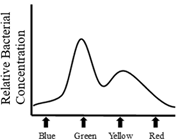
\includegraphics[width=\linewidth]{fig21.png}
                \caption*{}
                \label{fig:a36c}
            \end{minipage}%
            \begin{minipage}{0.45\textwidth}
                \centering
      \item     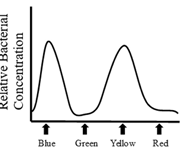
\includegraphics[width=\linewidth]{fig22.png}
                \caption*{}
                \label{fig:a36d}
            \end{minipage}
        \end{figure}
    \end{enumerate}

    \item Two RNAs shown below were used separately as templates in an in vitro translation system, which can generate proteins in all possible reading frames.
    \begin{align*}
        RNA_1 &: 5'-(AG)_n-3' \\
        RNA_2 &: 5'-(AAG)_n-3'
    \end{align*}
    The $RNA_1$ translated product contained Arg and Glu.
    The $RNA_2$ translated product contained Arg, Glu, and Lys.
    Which one of the following codons directs the incorporation of Arg?

    \hfill{\brak{\text{GATE XL 2022}}}
    \begin{enumerate}
        \begin{multicols}{4}
            \item AAG
            \item AGA
            \item GAA
            \item GAG
        \end{multicols}
    \end{enumerate}

    \item Which of the following statements about endogenous synthesis of insulin are correct?
    \begin{itemize}
        \item[P.] Insulin is synthesized as preproinsulin.
        \item[Q.] Preproinsulin is converted to proinsulin.
        \item[R.] Single-site cleavage of proinsulin eliminates C chain.
        \item[S.] Mature insulin consists of disulphide-linked A and B chains.
    \end{itemize}

    \hfill{\brak{\text{GATE XL 2022}}}
    \begin{enumerate}
        \begin{multicols}{2}
            \item P, Q, and R
            \item P, Q, and S
            \item P, R, and S
            \item Q, R, and S
        \end{multicols}
    \end{enumerate}

    \item Which one of the following enzymes converts testosterone to estradiol?

    \hfill{\brak{\text{GATE XL 2022}}}
    \begin{enumerate}
        \item Aromatase
        \item 3$\beta$-hydroxysteroid dehydrogenase
        \item 5$\alpha$-reductase
        \item 17$\beta$-hydroxysteroid dehydrogenase
    \end{enumerate}

    \item Purification of 6$\times$His-tagged protein using Ni-NTA column is an example of \underline{\hspace{2cm}}.

    \hfill{\brak{\text{GATE XL 2022}}}
    \begin{enumerate}
        \item affinity chromatography
        \item hydrophobic-interaction chromatography
        \item ion-exchange chromatography
        \item size-exclusion chromatography
    \end{enumerate}

    \item Which of the following carbohydrates has/have a $\beta1 \rightarrow 4$ glycosidic linkage?

    \hfill{\brak{\text{GATE XL 2022}}}
    \begin{enumerate}
        \begin{multicols}{2}
            \item Cellulose
            \item Chitin
            \item Lactose
            \item Maltose
        \end{multicols}
    \end{enumerate}

    \item Which of the following statements about IgA is/are correct?

    \hfill{\brak{\text{GATE XL 2022}}}
    \begin{enumerate}
        \item It is secreted into colostrum.
        \item It is transported across the cell by transcytosis.
        \item Its secretion is facilitated by poly-Ig receptor.
        \item It primarily exists as a dimer in serum.
    \end{enumerate}

    \item The standard free energy changes for conversion of phosphoenol pyruvate \brak{\text{PEP}} to pyruvate, and ATP synthesis are shown below.
    \begin{align*}
        PEP + H_2O &\rightleftharpoons pyruvate + P_i \quad \Delta G'^{\circ} = -61.9 \text{ kJ} \cdot \text{mol}^{-1} \\
        ADP + P_i &\rightleftharpoons ATP + H_2O \quad \Delta G'^{\circ} = 30.5 \text{ kJ} \cdot \text{mol}^{-1}
    \end{align*}
    The starting concentrations of PEP, ADP, pyruvate, and ATP are $25$, $25$, $50$, and $50$ mM, respectively. The value of universal gas constant \brak{\text{R}} is $8.315 \text{ J} \cdot \text{mol}^{-1}K^{-1}$. The actual free energy change in $\text{kJ} \cdot \text{mol}^{-1}$ for the reaction
    \[ PEP + ADP \rightarrow pyruvate + ATP \]
    carried out at $37\degree$C will be \underline{\hspace{2cm}} \brak{\text{rounded off to one place of decimal}}.

    \hfill{\brak{\text{GATE XL 2022}}}

    \item The dissociation constant for a receptor-ligand pair is $0.25 \times 10^{-7}$ M. The ligand was added to a solution of the receptor such that the receptor was $50\%$ saturated at equilibrium. Assume that the receptor has one ligand binding site. The concentration of the free ligand at equilibrium in nM, correct to the nearest integer, should be \underline{\hspace{2cm}}.

    \hfill{\brak{\text{GATE XL 2022}}}

    \item The half-maximal velocity of an enzyme catalyzed reaction was found at a substrate concentration of $0.5 \times 10^{-6}$ M. This enzyme follows Michaelis-Menten kinetics. In the presence of a competitive inhibitor, the half-maximal velocity was found at a substrate concentration of $1.5 \times 10^{-6}$ M. Given that the enzyme-inhibitor pair has a dissociation constant of $2 \times 10^{-7}$ M, the concentration of the competitive inhibitor in $\mu$M, rounded off to one place of decimal, was \underline{\hspace{2cm}}.

    \hfill{\brak{\text{GATE XL 2022}}}

    \item A forty-times diluted sample of ssRNA gave an $A_{260}$ of $0.01$. The concentration of the ssRNA before the dilution in $\mu$g/mL was \underline{\hspace{2cm}} \brak{\text{correct to the nearest integer}}.

    \hfill{\brak{\text{GATE XL 2022}}}

    \item In Angiosperms, normally 'Exarch Xylem' occurs in

    \hfill{\brak{\text{GATE XL 2022}}}
    \begin{enumerate}
        \begin{multicols}{2}
            \item dicot stem
            \item monocot stem
            \item dicot root
            \item dicot leaf
        \end{multicols}
    \end{enumerate}

    \item 'Quiescent Center' is present in

    \hfill{\brak{\text{GATE XL 2022}}}
    \begin{enumerate}
        \begin{multicols}{2}
            \item leaf meristem
            \item root apical meristem
            \item shoot apical meristem
            \item floral meristem
        \end{multicols}
    \end{enumerate}

    \item With reference to virulence \brak{\text{vir}} region of nopaline type Ti plasmid of \textit{Agrobacterium tumefaciens}, match Group-I \brak{\text{vir gene}} and Group-II \brak{\text{coded protein}} in CORRECT combination.
    \begin{table}[h!]
    \centering
    \caption*{}
    \label{tab:q49}
    \begin{tabular}{ll}
        \textbf{Group-I} & \textbf{Group-II} \\
        P. vir A & I. Single strand T-DNA binding protein \\
        Q. vir B & II. Topoisomerase \\
        R. vir E & III. Membrane protein, channel for T-DNA \\
        S. vir D & IV. Sensor protein, constitutive expression \\
    \end{tabular}
    \end{table}

    \hfill{\brak{\text{GATE XL 2022}}}
    \begin{enumerate}
        \begin{multicols}{2}
            \item P-IV, Q-III, R-II, S-I
            \item P-IV, Q-III, R-I, S-II
            \item P-IV, Q-II, R-I, S-III
            \item P-I, Q-III, R-II, S-IV
        \end{multicols}
    \end{enumerate}

    \item Anomalous secondary growth is observed in

    \hfill{\brak{\text{GATE XL 2022}}}
    \begin{enumerate}
        \begin{multicols}{4}
            \item Triticum
            \item Oryza
            \item Zea
            \item Dracaena
        \end{multicols}
    \end{enumerate}

    \item Which of the following plant diseases is/are caused by bacteria?

    \hfill{\brak{\text{GATE XL 2022}}}
    \begin{enumerate}
        \item Angular leaf spot of cotton
        \item Citrus canker
        \item Apple scab
        \item Leaf curl of papaya
    \end{enumerate}

    \item Phylogenetic system of classification is/are proposed by

    \hfill{\brak{\text{GATE XL 2022}}}
    \begin{enumerate}
        \item Carolus Linnaeus
        \item John Hutchinson
        \item Engler and Prantl
        \item Bentham and Hooker
    \end{enumerate}

    \item Which of the following is/are part of marine ecosystem?

    \hfill{\brak{\text{GATE XL 2022}}}
    \begin{enumerate}
        \item Open ocean
        \item Chaparral
        \item Deep sea
        \item Estuaries
    \end{enumerate}

    \item In NADP$^{+}$-malic enzyme type C$_4$ photosynthesis cycle, $n$ molecule\brak{\text{s}} of ATP is/are required for the assimilation of one molecule of CO$_2$. The value of $n$ is \underline{\hspace{2cm}} \brak{\text{in integer}}.

    \hfill{\brak{\text{GATE XL 2022}}}

    \item An \textit{Arabidopsis thaliana} mutant plant developed defective flowers with altered floral organ identity and patterning. In this mutant, the four floral whorls contain Sepal-Sepal-Carpel-Carpel, from the periphery to the center of the flower. Based on the typical ABC model of floral organ patterning, which among the following are mutated in this plant?

    \hfill{\brak{\text{GATE XL 2022}}}
    \begin{enumerate}
        \item Class A gene\brak{\text{s}}
        \item Class B gene\brak{\text{s}}
        \item Class C gene\brak{\text{s}}
        \item Double mutant for Class A and Class C genes
    \end{enumerate}

    \item Match the secondary metabolites in Group-I with types of secondary metabolites in Group-II in CORRECT order.
    \begin{table}[h!]
    \centering
    \caption*{}
    \label{tab:q56}
    \begin{tabular}{ll}
        \textbf{Group-I} & \textbf{Group-II} \\
        P. Myrcene & I. Sesquiterpene \\
        Q. $\beta$-Farnesene & II. Cyanogenic glycoside \\
        R. Amygdalin & III. Flavone \\
        S. Nicotine & IV. Alkaloid \\
        T. Luteolin & V. Monoterpene \\
    \end{tabular}
    \end{table}

    \hfill{\brak{\text{GATE XL 2022}}}
    \begin{enumerate}
        \begin{multicols}{2}
            \item P-I, Q-V, R-II, S-IV, T-III
            \item P-V, Q-II, R-IV, S-I, T-III
            \item P-II, Q-III, R-IV, S-V, T-I
            \item P-V, Q-I, R-II, S-IV, T-III
        \end{multicols}
     \end{enumerate}   

     \item Match Group-I \brak{\text{enzyme}}, Group-II \brak{\text{reaction catalyzed by the enzyme}}, and Group-III \brak{\text{subcellular localization of the enzyme and the associated metabolic process}} in CORRECT combination.

    \hfill{\brak{\text{GATE XL 2022}}}

    \begin{table}[h!]
    \centering
    \caption*{}
    \label{tab:q57}
    \begin{tabular}{lll}
    \hline
    \textbf{Group-I} & \textbf{Group-II} & \textbf{Group-III} \\
    \hline
    P. PEP Carboxylase & I. $2 \text{ Glycolate} + 2O_2 \rightarrow 2 \text{ Glyoxylate} + 2 H_2O_2$ & a. Cytosol - C4 cycle \\
    Q. Rubisco & II. $\text{Pyruvate} + \text{NAD}^+ + \text{CoA} \rightarrow \text{Acetyl-CoA} + CO_2 + \text{NADH}$ & b. Peroxisome - $C_2$ cycle \\
    R. Glycolate oxidase & III. $\text{Phosphoenolpyruvate} + HCO_3^- \rightarrow \text{Oxaloacetate} + P_i$ & c. Mitochondria - aerobic respiration \\
    S. Pyruvate dehydrogenase & IV. $3 \brak{\text{Ribulose 1,5-bisphosphate}} + 3 CO_2 + 3 H_2O \rightarrow 6 \brak{\text{3-phosphoglycerate}} + 6 H^+$ & d. Chloroplast - $C_3$ cycle \\
    \hline
    \end{tabular}
    \end{table}

    \begin{enumerate}
        \begin{multicols}{2}
        \item P-III-a, Q-IV-d, R-I-b, S-II-c
        \item P-II-a, Q-III-d, R-I-b, S-IV-c
        \item P-IV-a, Q-II-b, R-I-d, S-III-c
        \item P-IV-a, Q-II-d, R-I-b, S-III-c
        \end{multicols}
    \end{enumerate}

    \item Match Group-I \brak{\text{selection agent}} and Group-II \brak{\text{gene}} in CORRECT combination.

    \hfill{\brak{\text{GATE XL 2022}}}

    \begin{table}[h!]
    \centering
    \caption*{}
    \label{tab:q58}
    \begin{tabular}{ll}
    \hline
    \textbf{Group-I} & \textbf{Group-II} \\
    \hline
    P. Kanamycin & I. pmi \\
    Q. Hygromycin & II. bar \\
    R. Phosphinothricin & III. nptII \\
    S. Mannose & IV. ptxD \\
     & V. dhfr \\
     & VI. hpt \\
    \hline
    \end{tabular}
    \end{table}

    \begin{enumerate}
        \begin{multicols}{2}
        \item P-III, Q-VI, R-II, S-I
        \item P-IV, Q-III, R-II, S-I
        \item P-I, Q-VI, R-III, S-II
        \item P-II, Q-I, R-V, S-VI
        \end{multicols}
    \end{enumerate}

    \item Match Group I \brak{\text{plant natural product}}, Group II \brak{\text{class}} and Group III \brak{\text{source plant}} in CORRECT combination.

    \hfill{\brak{\text{GATE XL 2022}}}

    \begin{table}[h!]
    \centering
    \caption*{}
    \label{tab:q59}
    \begin{tabular}{lll}
    \hline
    \textbf{Group-I} & \textbf{Group-II} & \textbf{Group-III} \\
    \hline
    P. Reserpine & I. Stilbenes & a. Manihot esculanta \\
    Q. Resveratrol & II. Cyanogenic glycoside & b. Crocus sativus \\
    R. Picrocrocin & III. Alkaloid & c. Vitis vinifera \\
    S. Linamarin & IV. Monoterpene glycoside & d. Rauwolfia serpentina \\
    \hline
    \end{tabular}
    \end{table}

    \begin{enumerate}
        \begin{multicols}{2}
        \item P-I-d, Q-II-c, R-IV-a, S-III-b
        \item P-III-d, Q-IV-b, R-I-c, S-II-a
        \item P-II-a, Q-III-b, R-I-d, S-IV-c
        \item P-III-d, Q-I-c, R-IV-b, S-II-a
        \end{multicols}
    \end{enumerate}

    \item Match Group I \brak{\text{plant disease}}, Group II \brak{\text{causal organism}} and Group III \brak{\text{affected plant}} in CORRECT combination.

    \hfill{\brak{\text{GATE XL 2022}}}

    \begin{table}[h!]
    \centering
    \caption*{}
    \label{tab:q60}
    \begin{tabular}{lll}
    \hline
    \textbf{Group-I} & \textbf{Group-II} & \textbf{Group-III} \\
    \hline
    P. Karnal Bunt & I. Phytophthora infestans & a. Rice \\
    Q. Ergot & II. Blumeria graminis & b. Potato \\
    R. Late blight & III. Neovossia indica & c. Rye \\
    S. Powdery mildew & IV. Puccinia recondita & d. Wheat \\
     & V. Claviceps purpurea & e. Barley \\
     & VI. Alternaria solani & f. Brinjal \\
    \hline
    \end{tabular}
    \end{table}

    \begin{enumerate}
        \begin{multicols}{2}
        \item P-II-a, Q-V-b, R-III-d, S-I-e
        \item P-III-d, Q-V-c, R-II-e, S-IV-f
        \item P-III-d, Q-V-c, R-I-b, S-II-e
        \item P-V-c, Q-I-d, R-VI-b, S-II-e
        \end{multicols}
    \end{enumerate}

    \item Make CORRECT match between Group-I and Group-II, in relation to interaction between two species.

    \hfill{\brak{\text{GATE XL 2022}}}

    \begin{table}[h!]
    \centering
    \caption*{}
    \label{tab:q61}
    \begin{tabular}{ll}
    \hline
    \textbf{Group-I} & \textbf{Group-II} \\
    \hline
    P. Neutralism & I. neither can survive under natural condition without the other \\
    Q. Allelopathy & II. direct inhibition of one species by the other species using toxic compound \\
    R. Amensalism & III. neither is affected by the association with the other \\
    S. Mutualism & IV. one is inhibited and the other is not affected \\
    \hline
    \end{tabular}
    \end{table}

    \begin{enumerate}
        \begin{multicols}{2}
        \item P-I, Q-II, R-III, S-IV
        \item P-III, Q-II, R-IV, S-I
        \item P-IV, Q-III, R-II, S-I
        \item P-III, Q-IV, R-II, S-I
        \end{multicols}
    \end{enumerate}

    \item Which of the following matches is/are CORRECT?

    \hfill{\brak{\text{GATE XL 2022}}}

    \begin{enumerate}
        \item Surface fibre - Cotton - Gossypium hirsutum
        \item Bast fibre - Flax - Corchorus capsularis
        \item Drying oil - Safflower oil - Helianthus annuus
        \item Nondrying-oil - Castor oil - Ricinus communis
    \end{enumerate}

    \item Which of the following is/are phanerogamic parasite\brak{\text{s}}?

    \hfill{\brak{\text{GATE XL 2022}}}

    \begin{enumerate}
        \item Cuscuta reflexa
        \item Orobanche cernua
        \item Ocimum sanctum
        \item Santalum album
    \end{enumerate}

    \item When a true breeding tall plant containing red flowers was crossed with the true breeding dwarf plant containing white flowers, all F1 plants were tall with red flowers. When the F1 plant was self-pollinated, considering independent assortment of plant height and flower colour traits, the calculated percentage probability of dwarf plants bearing red flowers in the F2 generation is \underline{\hspace{2cm}} percent \brak{\text{round off to 2 decimal places}}.

    \hfill{\brak{\text{GATE XL 2022}}}

    \item A hypothetical plant gene ADSH22 is encoded by the nuclear genome. The length of the mature mRNA for ADSH22 is $2150$ nucleotides \brak{\text{nts}}. This mRNA has a $270$ nts long 5' UTR and $200$ nts long 3' UTR. Taking average molecular weight of an amino acid as $115$ Dalton \brak{\text{Da}}, the calculated molecular weight of ADSH22 protein is \underline{\hspace{2cm}} kDa \brak{\text{round off to 1 decimal place}}.

    \hfill{\brak{\text{GATE XL 2022}}}

    \item The terminal acceptor of electron during anaerobic respiration in Methanococcus is

    \hfill{\brak{\text{GATE XL 2022}}}

    \begin{enumerate}
        \begin{multicols}{2}
        \item Nitrate ion
        \item Sulfate ion
        \item Carbon dioxide
        \item Oxygen
        \end{multicols}
    \end{enumerate}

    \item Which one of the following mutagens convert DNA's adenine to hypoxanthine?

    \hfill{\brak{\text{GATE XL 2022}}}

    \begin{enumerate}
        \begin{multicols}{2}
        \item Ultraviolet light
        \item Mitomycin C
        \item Methyl methanesulfonate
        \item Nitrous acid
        \end{multicols}
    \end{enumerate}

    \item Which one of the following leukocytes are present in the largest proportion in healthy human blood?

    \hfill{\brak{\text{GATE XL 2022}}}

    \begin{enumerate}
        \begin{multicols}{2}
        \item Neutrophils
        \item Eosinophils
        \item Basophiles
        \item Monocytes
        \end{multicols}
    \end{enumerate}

    \item The site of photosynthesis in cyanobacteria is

    \hfill{\brak{\text{GATE XL 2022}}}

    \begin{enumerate}
        \begin{multicols}{2}
        \item Chloroplast
        \item Chromatophores
        \item Thylakoids
        \item Chlorosomes
        \end{multicols}
    \end{enumerate}

    \item The antimicrobial activity of vancomycin is due to the

    \hfill{\brak{\text{GATE XL 2022}}}

    \begin{enumerate}
        \item inhibition of nucleic acid synthesis
        \item damage to the cytoplasmic membrane
        \item inhibition of cell wall synthesis
        \item regulation of DNA supercoiling
    \end{enumerate}

    \item Phenolics act as disinfectant by

    \hfill{\brak{\text{GATE XL 2022}}}

    \begin{enumerate}
        \item rupturing plasma membrane followed by leakage of cellular contents
        \item bond formation between adjacent pyrimidine bases
        \item forming adduct with amino acid and unsaturated fatty acids
        \item alkylation of proteins
    \end{enumerate}

    \item Which of the following methods are used for the identification of microorganisms?

    \hfill{\brak{\text{GATE XL 2022}}}

    \begin{enumerate}
        \item Nucleic acid hybridization
        \item Southern blotting
        \item 16s rRNA sequencing
        \item Percentage G-C content
    \end{enumerate}

    \item Which of the following are present in Gram-negative bacteria?

    \hfill{\brak{\text{GATE XL 2022}}}

    \begin{enumerate}
        \item Lipopolysaccharide
        \item Teichoic acid
        \item Periplasm
        \item Endotoxin
    \end{enumerate}

    \item Nonsense suppressor mutation is found in \underline{\hspace{2cm}}.

    \hfill{\brak{\text{GATE XL 2022}}}

    \begin{enumerate}
        \begin{multicols}{2}
        \item rRNA
        \item tRNA
        \item start codon of mRNA
        \item stop codon of mRNA
        \end{multicols}
    \end{enumerate}

    \item Choose the correct match for structural components of bacteria to their function.

    \hfill{\brak{\text{GATE XL 2022}}}

    \begin{table}[h!]
    \centering
    \caption*{}
    \label{tab:q75}
    \begin{tabular}{ll}
    \hline
    \textbf{Structural component} & \textbf{Function} \\
    \hline
    (P) Flagella & (i) prevent cell lysis \\
    (Q) Cell wall & (ii) chemotaxis \\
    (R) Metachromatic granules & (iii) storage for ATP \\
    (S) Magnetosomes & (iv) cell orientation \\
    \hline
    \end{tabular}
    \end{table}

    \begin{enumerate}
        \item (P)-(ii), (Q)-(iii), (R)-(i), (S)-(iv)
        \item (P)-(ii), (Q)-(i), (R)-(iii), (S)-(iv)
        \item (P)-(ii), (Q)-(i), (R)-(iv), (S)-(iii)
        \item (P)-(i), (Q)-(iv), (R)-(iii), (S)-(ii)
    \end{enumerate}

    \item Match the pathogen with the appropriate disease.

    \hfill{\brak{\text{GATE XL 2022}}}

    \begin{table}[h!]
    \centering
    \caption*{}
    \label{tab:q76}
    \begin{tabular}{ll}
    \hline
    \textbf{Pathogen} & \textbf{Disease} \\
    \hline
    (P) Streptococcus pyogenes & (i) Scarlet fever \\
    (Q) Brucella species & (ii) Pott’s disease \\
    (R) Mycobacterium tuberculosis & (iii) Traveler’s diarrhea \\
    (S) Escherichia coli & (iv) Undulant fever \\
    \hline
    \end{tabular}
    \end{table}

    \begin{enumerate}
        \item (P)-(ii), (Q)-(iii), (R)-(i), (S)-(iv)
        \item (P)-(ii), (Q)-(i), (R)-(iii), (S)-(iv)
        \item (P)-(i), (Q)-(iv), (R)-(ii), (S)-(iii)
        \item (P)-(i), (Q)-(iv), (R)-(iii), (S)-(ii)
    \end{enumerate}

    \item Match the correct mode of cell division with respective bacteria.

    \hfill{\brak{\text{GATE XL 2022}}}
 \textbf{Mode of cell division}   
    \begin{figure}[h!]
        \centering
        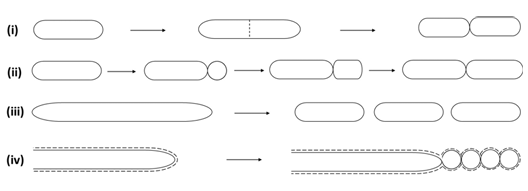
\includegraphics[width=0.8\columnwidth]{fig23.png}
        \caption*{}
        \label{fig:q77}
    \end{figure}

    \textbf{Bacteria}
\begin{enumerate}[label=\textbf{\Alph*}),start=16]
  \item Streptomyces species 
  \item  Rhodopseudomonas acidophila 
  \item  Bacillus subtilis 
  \item  Nocardia species
    \end{enumerate}

    \begin{enumerate}
        \item (P)-(ii), (Q)-(iii), (R)-(i), (S)-(iv)
        \item (P)-(ii), (Q)-(i), (R)-(iii), (S)-(iv)
        \item (P)-(iv), (Q)-(ii), (R)-(i), (S)-(iii)
        \item (P)-(i), (Q)-(iv), (R)-(iii), (S)-(ii)
    \end{enumerate}

    \item The correct sequence of overall biochemical reaction which expresses the process of denitrification is \underline{\hspace{2cm}}

    \hfill{\brak{\text{GATE XL 2022}}}

    \begin{enumerate}
        \item $2\text{NO}_3^- \rightarrow 2\text{NO}_2^- \rightarrow \text{N}_2\text{O} \rightarrow 2\text{NO} \rightarrow \text{N}_2$
        \item $2\text{NO}_3^- \rightarrow 2\text{NO}_2^- \rightarrow 2\text{NO} \rightarrow \text{N}_2\text{O} \rightarrow \text{N}_2$
        \item $2\text{NO}_3^- \rightarrow 2\text{NO} \rightarrow 2\text{NO}_2^- \rightarrow \text{N}_2\text{O} \rightarrow \text{N}_2$
        \item $2\text{NO}_3^- \rightarrow \text{N}_2\text{O} \rightarrow 2\text{NO} \rightarrow 2\text{NO}_2^- \rightarrow \text{N}_2$
    \end{enumerate}

    \item Which of the following diseases are caused by family of DNA viruses?

    \hfill{\brak{\text{GATE XL 2022}}}

    \begin{enumerate}
        \item Hepatitis B
        \item Smallpox
        \item Influenza
        \item Rabies
    \end{enumerate}

    \item Which of the following Gram-positive cocci are found in biofilm of dental plaque?

    \hfill{\brak{\text{GATE XL 2022}}}

    \begin{enumerate}
        \item Gonococcus
        \item Streptococcus mutans
        \item Streptococcus sobrinus
        \item Fusobacterium species
    \end{enumerate}

    \item Which of the following statements are TRUE for archaea?

    \hfill{\brak{\text{GATE XL 2022}}}

    \begin{enumerate}
        \item Cell wall in archaea contains muramic acid and D-amino acid
        \item N-Formylmethionine is the first amino acid to initiate new polypeptide chain synthesis in archaea
        \item Methionine is the first amino acid used during protein synthesis in archaea
        \item Membrane of archaea contains phytanyl rather than fatty acids
    \end{enumerate}

    \item If the plasmid given below is digested with restriction enzymes HindIII and EcoRI, considering complete digestion, how many DNA fragments will be released?

    \hfill{\brak{\text{GATE XL 2022}}}
    
    \begin{figure}[h!]
        \centering
        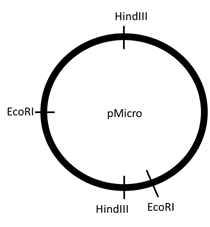
\includegraphics[width=0.4\columnwidth]{fig24.png}
        \caption*{}
        \label{fig:q82}
    \end{figure}

    \item Escherichia coli growing under favorable conditions doubles in every $20$ minutes. If the initial number of Escherichia coli cells is $100$, what will be the logarithmic number of cells at $17^{th}$ generation? \brak{\text{Answer up to 1 decimal place}}

    \hfill{\brak{\text{GATE XL 2022}}}

    \item What will be value of the Numerical Aperture \brak{\text{NA}}, if half aperture angle is $58\degree$ and oil immersed objective is used for the process of light microscopy? \brak{\text{Answer up to 1 decimal place}} Consider $\sin 58\degree = 0.85$ and refractive index of immersion oil used is $= 1.50$.

    \hfill{\brak{\text{GATE XL 2022}}}

    \item Which one of the following organic compounds is composed of only \brak{\text{i}} a nitrogen containing base, \brak{\text{ii}} a single five-carbon sugar, and \brak{\text{iii}} a triphosphate?

    \hfill{\brak{\text{GATE XL 2022}}}
    \begin{enumerate}
        \item Nucleoside
        \item Nucleotide
        \item Base
        \item Nucleic acid
    \end{enumerate}

    \item Which one of the following animals develops adaptive predator avoidance morphology because of the presence of high predator number in its habitat?

    \hfill{\brak{\text{GATE XL 2022}}}
    \begin{enumerate}
        \item Daphnia sp.
        \item Scaphiopus sp.
        \item Wolbachia sp.
        \item Rhodnius sp.
    \end{enumerate}

    \item To which class of Drosophila developmental genes does fushi tarazu \brak{\text{ftz}} belong?

    \hfill{\brak{\text{GATE XL 2022}}}
    \begin{enumerate}
        \begin{multicols}{2}
        \item Gap genes
        \item Segment polarity genes
        \item Pair rule genes
        \item Maternal effect genes
        \end{multicols}
    \end{enumerate}

    \item The action of which class of enzyme inhibitors can be reversed by adding an excess of substrate?

    \hfill{\brak{\text{GATE XL 2022}}}
    \begin{enumerate}
        \begin{multicols}{2}
        \item Uncompetitive inhibitors
        \item Competitive inhibitors
        \item Non-specific inhibitors
        \item Allosteric inhibitors
        \end{multicols}
    \end{enumerate}

    \item Mendel deduced the genetic principle of inheritance by experimenting on sweet pea plants. One of the experiments involved crossing plants with two contrasting characters, tall \brak{\text{dominant}} and dwarf \brak{\text{recessive}}, which yielded all tall plants in the first generation. When the same genetic cross was independently repeated by a researcher, only short plants were obtained. Which one of the following can possibly explain the altered outcome?

    \hfill{\brak{\text{GATE XL 2022}}}
    \begin{enumerate}
        \item Tall plants were heterozygous
        \item An enhancer for the tall allele is present in the dwarf plant
        \item A suppressor for the tall allele is present in the dwarf plant
        \item Dwarf plants are homozygous
    \end{enumerate}

    \item Which of the following is/are responsible for reversible receptor-ligand interaction?

    \hfill{\brak{\text{GATE XL 2022}}}
    \begin{enumerate}
        \begin{multicols}{2}
        \item Ionic interactions
        \item Hydrogen bonding
        \item Peptide bonding
        \item Hydrophobic interactions
        \end{multicols}
    \end{enumerate}

    \item In the human body, which of the following is/are involved in processing of a foreign antigen?

    \hfill{\brak{\text{GATE XL 2022}}}
    \begin{enumerate}
        \begin{multicols}{2}
        \item B-cells
        \item Macrophages
        \item Red blood cells
        \item Platelets
        \end{multicols}
    \end{enumerate}

    \item Animals can be classified as 'specialists' or 'generalists' with respect to diet and habitat selection. Which of the following organism/s belong/s to the specialist category?

    \hfill{\brak{\text{GATE XL 2022}}}
    \begin{enumerate}
        \begin{multicols}{2}
        \item Raccoon
        \item Panda
        \item Polar Bear
        \item Koala Bear
        \end{multicols}
    \end{enumerate}

    \item Match the drug/chemicals listed in Column I with the developmental/physiological defects listed in Column II.

    \hfill{\brak{\text{GATE XL 2022}}}
    \begin{table}[h!]
    \centering
    \caption*{}
    \label{tab:q93}
    \begin{tabular}{ll}
    \hline
    \textbf{Column I} & \textbf{Column II} \\
    \hline
    P. Veratrum alkaloids & \brak{\text{i}} Obesity \\
    Q. Thalidomide & \brak{\text{ii}} Minamata syndrome \\
    R. Methylmercury & \brak{\text{iii}} Cyclopia \\
    S. Diethylstilbesterol & \brak{\text{iv}} Phocomelia \\
    \hline
    \end{tabular}
    \end{table}
    \begin{enumerate}
        \item P-\brak{\text{iii}}; Q-\brak{\text{iv}}; R-\brak{\text{ii}}; S-\brak{\text{i}}
        \item P-\brak{\text{i}}; Q-\brak{\text{iv}}; R-\brak{\text{iii}}; S-\brak{\text{ii}}
        \item P-\brak{\text{ii}}; Q-\brak{\text{iv}}; R-\brak{\text{iii}}; S-\brak{\text{i}}
        \item P-\brak{\text{ii}}; Q-\brak{\text{iii}}; R-\brak{\text{iv}}; S-\brak{\text{i}}
    \end{enumerate}

    \item Match the animals listed in Column I with primary tissue or organ of residence in the host listed in Column II

    \hfill{\brak{\text{GATE XL 2022}}}
    \begin{table}[h!]
    \centering
    \caption*{}
    \label{tab:q94}
    \begin{tabular}{ll}
    \hline
    \textbf{Column I} & \textbf{Column II} \\
    \hline
    P. Ascaris lumbricoides & \brak{\text{i}} Subcutaneous tissue in human \\
    Q. Dracunculus medinensis & \brak{\text{ii}} Lymphatic vessels and lymph nodes \\
    R. Enterobius vermicularis & \brak{\text{iii}} Small intestine \\
    S. Wuchereria bancrofti & \brak{\text{iv}} Caecum or vermiform appendix \\
    \hline
    \end{tabular}
    \end{table}
    \begin{enumerate}
        \begin{multicols}{2}
        \item P-\brak{\text{iii}}, Q-\brak{\text{iv}}, R-\brak{\text{ii}}, S-\brak{\text{i}}
        \item P-\brak{\text{i}}, Q-\brak{\text{iv}}, R-\brak{\text{iii}}, S-\brak{\text{ii}}
        \item P-\brak{\text{ii}}, Q-\brak{\text{iii}}, R-\brak{\text{iv}}, S-\brak{\text{i}}
        \item P-\brak{\text{iii}}, Q-\brak{\text{i}}, R-\brak{\text{iv}}, S-\brak{\text{ii}}
        \end{multicols}
    \end{enumerate}

    \item Match the cell types listed in Column I with their sources in Column II and the primary functional roles listed in Column III.

    \hfill{\brak{\text{GATE XL 2022}}}
    \begin{table}[h!]
    \centering
    \caption*{}
    \label{tab:q95}
    \begin{tabular}{lll}
    \hline
    \textbf{Column I} & \textbf{Column II} & \textbf{Column III} \\
    \hline
    P. Microglial cells & \brak{\text{i}} Lung & a. Visual transduction \\
    Q. Leydig cells & \brak{\text{ii}} Eyes & b. Hormone secretion \\
    R. ON cells & \brak{\text{iii}} Brain & c. Phagocytosis \\
    S. Pneumocytes & \brak{\text{iv}} Testis & d. Gaseous exchange \\
    \hline
    \end{tabular}
    \end{table}
    \begin{enumerate}
        \begin{multicols}{2}
        \item P-\brak{\text{iii}}-b, Q-\brak{\text{iv}}-c, R-\brak{\text{ii}}-a, S-\brak{\text{i}}-d
        \item P-\brak{\text{ii}}-c, Q-\brak{\text{iv}}-d, R-\brak{\text{i}}-a, S-\brak{\text{iii}}-b
        \item P-\brak{\text{i}}-a, Q-\brak{\text{iv}}-b, R-\brak{\text{ii}}-c, S-\brak{\text{iii}}-d
        \item P-\brak{\text{iii}}-c, Q-\brak{\text{iv}}-b, R-\brak{\text{ii}}-a, S-\brak{\text{i}}-d
        \end{multicols}
    \end{enumerate}

    \item Match the ecological concepts listed in Column I with their definitions listed in Column II.

    \hfill{\brak{\text{GATE XL 2022}}}
    \begin{table}[h!]
    \centering
    \caption*{}
    \label{tab:q96}
    \begin{tabular}{ll}
    \hline
    \textbf{Column I} & \textbf{Column II} \\
    \hline
    P. Dominance hierarchies & \brak{\text{i}} Giving up one's own reproductive potential to benefit another individual \\
    Q. Territory & \brak{\text{ii}} Selection acting on related animals which affects fitness of an individual \\
    R. Altruism & \brak{\text{iii}} Exclusion of competing individuals using agonistic behavior \\
    S. Kin selection & \brak{\text{iv}} Preferential access to the food and mates in a group \\
    \hline
    \end{tabular}
    \end{table}
    \begin{enumerate}
        \begin{multicols}{2}
        \item P-\brak{\text{ii}}, Q-\brak{\text{iv}}, R-\brak{\text{i}}, S-\brak{\text{iii}}
        \item P-\brak{\text{iv}}, Q-\brak{\text{ii}}, R-\brak{\text{i}}, S-\brak{\text{ii}}
        \item P-\brak{\text{iii}}, Q-\brak{\text{iv}}, R-\brak{\text{i}}, S-\brak{\text{ii}}
        \item P-\brak{\text{i}}, Q-\brak{\text{iv}}, R-\brak{\text{iii}}, S-\brak{\text{ii}}
        \end{multicols}
    \end{enumerate}

    \item Match the hormones listed in Column I with their primary source tissues in Column II and the primary target tissues listed in Column III

    \hfill{\brak{\text{GATE XL 2022}}}
    \begin{table}[h!]
    \centering
    \caption*{}
    \label{tab:q97}
    \begin{tabular}{lll}
    \hline
    \textbf{Column I} & \textbf{Column II} & \textbf{Column III} \\
    \hline
    P. Epinephrine & \brak{\text{i}} Hypothalamus & a. Pituitary \\
    Q. Prolactin & \brak{\text{ii}} Thyroid & b. Heart \\
    R. Calcitonin & \brak{\text{iii}} Pituitary & c. Bone \\
    S. Thyrotropin releasing hormone & \brak{\text{iv}} Chromaffin tissue & d. Pigeon's crop \\
    \hline
    \end{tabular}
    \end{table}
    \begin{enumerate}
        \begin{multicols}{2}
        \item P-\brak{\text{iii}}-b, Q-\brak{\text{iv}}-c, R-\brak{\text{ii}}-a, S-\brak{\text{i}}-d
        \item P-\brak{\text{iv}}-c, Q-\brak{\text{iii}}-b, R-\brak{\text{ii}}-a, S-\brak{\text{i}}-d
        \item P-\brak{\text{iv}}-b, Q-\brak{\text{iii}}-d, R-\brak{\text{ii}}-c, S-\brak{\text{i}}-a
        \item P-\brak{\text{iii}}-b, Q-\brak{\text{iv}}-c, R-\brak{\text{ii}}-d, S-\brak{\text{i}}-a
        \end{multicols}
    \end{enumerate}

    \item 2-Deoxyglucose \brak{\text{2-DG}} inhibits the proliferation of cells and hence finds use as an anti-cancer agent. It is also used in COVID therapy, where it blocks hyperproliferation of virus-infected cells. Mechanistically, 2-DG blocks glycolysis by inhibiting the activities of which of the following enzyme/s?

    \hfill{\brak{\text{GATE XL 2022}}}
    \begin{enumerate}
        \begin{multicols}{2}
        \item Hexokinase
        \item Glucose 6-phosphate isomerase
        \item Glucose-6 phosphate dehydrogenase
        \item Phosphofructokinase
        \end{multicols}
    \end{enumerate}

    \item According to Abbe's equation on microscopy, the ability to resolve two entities inside a cell by light microscopy depends on which of the following factor/s?

    \hfill{\brak{\text{GATE XL 2022}}}
    \begin{enumerate}
        \begin{multicols}{2}
        \item Magnification of the objective lens
        \item Intensity of incident light
        \item Wavelength
        \item Numerical aperture of the objective lens
        \end{multicols}
    \end{enumerate}

    \item Match the animal inactivity behaviors listed in Column I with representative animals in Column II and their definitions listed in Column III.

    \hfill{\brak{\text{GATE XL 2022}}}
    \begin{table}[h!]
    \centering
    \caption*{}
    \label{tab:q100}
    \begin{tabular}{lll}
    \hline
    \textbf{Column I} & \textbf{Column II} & \textbf{Column III} \\
    \hline
    P. Torpor & \brak{\text{i}} Australian burrowing frogs & a. Prolonged period of inactivity without reducing body temperature \\
    Q. Hibernation & \brak{\text{ii}} Polar Bears & b. Inactivity period which accompanies extended periods of dryness \\
    R. Winter sleep & \brak{\text{iii}} Ground Squirrels & c. Decreased metabolism with lowered body temperature occurring in daily activity cycles \\
    S. Aestivation & \brak{\text{iv}} Hummingbirds & d. Decreased metabolism and lower body temperature for weeks or months \\
    \hline
    \end{tabular}
    \end{table}
    \begin{enumerate}
        \begin{multicols}{2}
        \item P-\brak{\text{ii}}-c, Q-\brak{\text{iv}}-b, R-\brak{\text{i}}-a, S-\brak{\text{iii}}-d
        \item P-\brak{\text{iv}}-c, Q-\brak{\text{iii}}-d, R-\brak{\text{ii}}-a, S-\brak{\text{i}}-b
        \item P-\brak{\text{iv}}-c, Q-\brak{\text{ii}}-b, R-\brak{\text{i}}-a, S-\brak{\text{iii}}-d
        \item P-\brak{\text{iv}}-b, Q-\brak{\text{i}}-c, R-\brak{\text{ii}}-d, S-\brak{\text{iii}}-a
        \end{multicols}
    \end{enumerate}

    \item If the vital capacity \brak{\text{VC}} of an individual is $4900$ ml, the tidal volume \brak{\text{TV}} is $500$ ml, and the inspiratory reserve volume \brak{\text{IRV}} is $3300$ ml, the expiratory reserve volume \brak{\text{ERV}} of the individual is \underline{\hspace{2cm}} ml \brak{\text{in integer}}.

    \hfill{\brak{\text{GATE XL 2022}}}

    \item A typical food chain involves producers, herbivores, primary carnivores and secondary carnivores. Based on Lindeman’s law of trophic efficiency, if producers have $40$ kJ of energy, the energy that will be stored in secondary carnivores is \underline{\hspace{2cm}} kJ \brak{\text{round off to two decimal places}}.

    \hfill{\brak{\text{GATE XL 2022}}}

    \item The average body length of Drosophila nasuta collected from Andaman and Nicobar Islands is 2 mm. From this population, a few males and females having a body length of 3 mm were selected and interbred. The average body length of the resultant progeny was 2.5 mm. The heritability {$h^2$} of the body length in this population is \underline{\hspace{2cm}}.
    \brak{\text{round off to one decimal place}}

    \hfill{\brak{\text{GATE XL 2022}}}

    \item Which among the given options truly depict the lines 1 and 2 in the figure below with respect to the effect of heat processing on food?

    \hfill{\brak{\text{GATE XL 2022}}}
    \begin{figure}[h!]
    \centering
    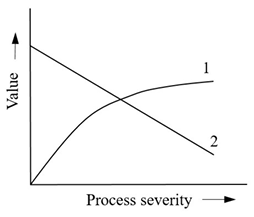
\includegraphics[width=0.4\columnwidth]{fig25.png}
    \caption*{}
    \label{fig:q104}
    \end{figure}
    \begin{enumerate}
        \begin{multicols}{2}
        \item 1-Safety, 2-Quality
        \item 1-Yield, 2-Safety
        \item 1-Yield, 2-Quality
        \item 1-Quality, 2-Safety
        \end{multicols}
    \end{enumerate}

    \item Homogenization of milk leads to disintegration of fat globules by

    \hfill{\brak{\text{GATE XL 2022}}}
    \begin{enumerate}
        \item Turbulence and pasteurization
        \item Pasteurization and cavitation
        \item Pasteurization and pressurization
        \item Turbulence and cavitation
    \end{enumerate}

    \item The lowest water activity {$a_w$} supporting the growth of Staphylococcus aureus in food under aerobic condition is

    \hfill{\brak{\text{GATE XL 2022}}}
    \begin{enumerate}
        \begin{multicols}{2}
        \item $0.98$
        \item $0.91$
        \item $0.89$
        \item $0.86$
        \end{multicols}
    \end{enumerate}

    \item Cultures used in industrial production of yogurt are

    \hfill{\brak{\text{GATE XL 2022}}}
    \begin{enumerate}
        \item Lactococcus lactis subsp. lactis
        \item Streptococcus thermophilus
        \item Leuconostoc mesenteroides subsp. cremoris
        \item Lactobacillus delbrueckii subsp. bulgaricus
    \end{enumerate}

    \item In a dairy plant, spray drying technology is used to produce whey powder. The rate of spray drying depends on

    \hfill{\brak{\text{GATE XL 2022}}}
    \begin{enumerate}
        \begin{multicols}{2}
        \item Temperature of the incoming air
        \item Shape of the cyclone separator
        \item Diameter of the whey droplet
        \item Heat transfer coefficient of hot air
        \end{multicols}
    \end{enumerate}

    \item The parboiling of paddy results into

    \hfill{\brak{\text{GATE XL 2022}}}
    \begin{enumerate}
        \begin{multicols}{2}
        \item Increase in the milling losses
        \item Increase in the nutritional value of rice
        \item Increase in the head rice recovery
        \item Increase in the broken rice percentage
        \end{multicols}
    \end{enumerate}

    \item One hundred kg paddy is dried from $18\%$ wet basis to $13\%$ wet basis moisture content. The amount of water removed \brak{\text{in kg}} from the paddy is \underline{\hspace{2cm}} \brak{\text{round off to one decimal place}}.

    \hfill{\brak{\text{GATE XL 2022}}}

    \item In a canning industry, the total process time {$F_0$} was calculated as $3$ min. If each can contains $20$ spores having decimal reduction time of $1.6$ min, the probability of spoilage would be \underline{\hspace{2cm}} in $100$ cans \brak{\text{round off to the nearest integer}}.

    \hfill{\brak{\text{GATE XL 2022}}}

    \item Match the edible oil refining stages given in Column I with their respective functions in Column II

    \hfill{\brak{\text{GATE XL 2022}}}
    \begin{table}[h!]
    \centering
    \caption*{}
    \label{tab:q112}
    \begin{tabular}{ll}
    \hline
    \textbf{Column I} & \textbf{Column II} \\
    \hline
    P. Degumming & 1. Separation of waxes \\
    Q. Neutralization & 2. Removal of pigments \\
    R. Bleaching & 3. Removal of phosphatides \\
    S. Winterization & 4. Removal of free fatty acids \\
    \hline
    \end{tabular}
    \end{table}
    \begin{enumerate}
        \begin{multicols}{2}
        \item P-3, Q-2, R-1, S-4
        \item P-2, Q-1, R-3, S-4
        \item P-3, Q-4, R-2, S-1
        \item P-3, Q-1, R-2, S-4
        \end{multicols}
    \end{enumerate}

    \item Make the correct pair of food packaging technology given in Column I with operating principle or description in Column II.

    \hfill{\brak{\text{GATE XL 2022}}}
    \begin{table}[h!]
    \centering
    \caption*{}
    \label{tab:q113}
    \begin{tabular}{ll}
    \hline
    \textbf{Column I} & \textbf{Column II} \\
    \hline
    P. Aseptic packaging & 1. Control of the concentration of $O_2$ and $CO_2$ inside the package \\
    Q. Active packaging & 2. Create a skin tight package wall \\
    R. Modified atmosphere packaging & 3. Independent sterilization of food and packaging material and \\
     & packaging under sterile environment \\
    S. Vacuum packaging & 4. Makes non-passive contribution to product development \\
    \hline
    \end{tabular}
    \end{table}
    \begin{enumerate}
        \begin{multicols}{2}
        \item P-3, Q-4, R-1, S-2
        \item P-3, Q-2, R-1, S-4
        \item P-1, Q-4, R-3, S-2
        \item P-3, Q-1, R-4, S-2
        \end{multicols}
    \end{enumerate}

    \item Which of the following is not a caramel flavour producing compound?

    \hfill{\brak{\text{GATE XL 2022}}}
    \begin{enumerate}
        \begin{multicols}{2}
        \item 3-Hydroxy-2-methylpyran-4-one
        \item 2H-4-Hydroxy-5-methylfuran-3-one
        \item 3-Hydroxy-2-acetylfuran
        \item p-Amino benzoicacid
        \end{multicols}
    \end{enumerate}

    \item Match the size reduction equipment in Column I with the method of operation in Column II.

    \hfill{\brak{\text{GATE XL 2022}}}
    \begin{table}[h!]
    \centering
    \caption*{}
    \label{tab:q115}
    \begin{tabular}{ll}
    \hline
    \textbf{Column I} & \textbf{Column II} \\
    \hline
    P. Hammer mill & 1. Compression \\
    Q. Burr mill & 2. Impact \\
    R. Crushing rolls & 3. Cutting \\
    S. Rotary knife & 4. Attrition \\
    \hline
    \end{tabular}
    \end{table}
    \begin{enumerate}
        \begin{multicols}{2}
        \item P-2, Q-4, R-1, S-3
        \item P-3, Q-1, R-2, S-4
        \item P-4, Q-1, R-2, S-3
        \item P-3, Q-4, R-2, S-1
        \end{multicols}
    \end{enumerate}

    \item Most commonly used refrigerant in direct immersion freezing of food is

    \hfill{\brak{\text{GATE XL 2022}}}
    \begin{enumerate}
        \begin{multicols}{2}
        \item Monochlorodifluoromethane
        \item Dichlorodifluoromethane
        \item Liquid nitrogen
        \item Freon
        \end{multicols}
    \end{enumerate}

    \item Which among the following are $\omega-6$ poly unsaturated essential fatty acids?

    \hfill{\brak{\text{GATE XL 2022}}}
    \begin{enumerate}
        \begin{multicols}{2}
        \item Linoleic acid
        \item ${\alpha}$-Linolenic acid
        \item ${\gamma}$-Linolenic acid
        \item Arachidonic acid
        \end{multicols}
    \end{enumerate}

    \item Which among the following statements are true with respect to protein denaturation?

    \hfill{\brak{\text{GATE XL 2022}}}
    \begin{enumerate}
        \item There may be an increase in $\alpha$-helix and $\beta$-sheet structure
        \item It is an irreversible process
        \item When fully denatured, globular proteins resemble a random coil
        \item The peptide bonds are broken
    \end{enumerate}

    \item Identify the correct pair\brak{\text{s}} of milling equipment and the grain for which it is used.

    \hfill{\brak{\text{GATE XL 2022}}}
    \begin{enumerate}
        \begin{multicols}{2}
        \item Mist polisher–Rice
        \item Break roll–Wheat
        \item Rubber roll–Pigeon pea
        \item Beall degermer–Maize
        \end{multicols}
    \end{enumerate}

    \item Which among the following expression\brak{\text{s}} is/are correct?

    \hfill{\brak{\text{GATE XL 2022}}}
    \begin{enumerate}
        \item Reynolds number = $\frac{\text{Density} \times \text{Velocity} \times \text{Characteristic dimension}}{\text{Viscosity}}$
        \item Nusselt number = $\frac{\text{Convective heat transfer coefficient} \times \text{Characteristic dimension}}{\text{Thermal conductivity of solid}}$
        \item Schmidt number = $\frac{\text{Kinematic viscosity of fluid}}{\text{Diffusivity}}$
        \item Biot number = $\frac{\text{Convective heat transfer coefficient} \times \text{Characteristic dimension}}{\text{Thermal conductivity of fluid}}$
    \end{enumerate}

    \item In a dairy processing plant, milk enters a $30$ m long and $2$ cm diameter tube at $60 \degree C$ and leaves at $57 \degree C$. The total heat loss over the tube length is $381.15$ W. The specific heat capacity, density, and viscosity of milk are $3.85$ kJ kg$^{-1}$ K$^{-1}$, $1020$ kg m$^{-3}$, and $1.20$ cP, respectively. The Reynolds number for the flow is \underline{\hspace{2cm}} \brak{\text{round off to the nearest integer}}.
    
    \hfill{\brak{\text{GATE XL 2022}}}
    
    Given: $\pi = 3.14$
    
    \item The dry bulb temperature and relative humidity of air inside a storage chamber are $37 \degree C$ and $50\%$, respectively. The saturation pressure of water vapour at $37 \degree C$ and barometric pressure are $6.28$ kPa and $101.32$ kPa, respectively. The humidity ratio of air inside the chamber is \underline{\hspace{2cm}} kg water \brak{\text{kg dry air}}$^{-1}$ \brak{\text{round off to three decimal places}}.
    
    \hfill{\brak{\text{GATE XL 2022}}}
    
    Given: Molecular weight of water vapour and dry air are $18.02$ g mol$^{-1}$ and $28.97$ g mol$^{-1}$, respectively.
    
\end{enumerate}

\end{document}

